\documentclass[12pt,a4paper]{article}

% ── Packages ──────────────────────────────────────────────
\usepackage[utf8]{inputenc}
\usepackage[T1]{fontenc}
\usepackage{lmodern}
\usepackage{amsmath,amssymb,amsthm}
\usepackage{mathtools}
\usepackage{geometry}
\geometry{margin=1in}
\usepackage{graphicx}
\graphicspath{{figures/}}
\usepackage{booktabs}
\usepackage{hyperref}
\hypersetup{
    colorlinks=true,
    linkcolor=blue!60!black,
    citecolor=blue!60!black,
    urlcolor=blue!60!black
}
\usepackage{caption}
\usepackage{float}
\usepackage{enumitem}
\usepackage{xcolor}

% ── Custom commands ───────────────────────────────────────
\newcommand{\Hfour}{H_4}
\newcommand{\Hthree}{H_3}
\newcommand{\Eeight}{E_8}
\newcommand{\vphi}{\varphi}
\newcommand{\Lmat}{L_{H_4}}
\newcommand{\R}{\mathbb{R}}
\newcommand{\Q}{\mathbb{Q}}
\newcommand{\Z}{\mathbb{Z}}

\newtheorem{definition}{Definition}
\newtheorem{observation}{Observation}

% ── Title ─────────────────────────────────────────────────
\title{%
  \textbf{Attractor Invariants and Scaling Relations\\
  in the $\Hfour$ System}\\[6pt]
  \large Part~V of a Series on Symmetry-Constrained Resonant Structure%
}
\author{%
  Lee Smart\\[4pt]
  \textit{Institute of Vibrational Field Dynamics}\\[2pt]
  \texttt{contact@vibrationalfielddynamics.org}\\[2pt]
  \texttt{@vfd\_org}%
}
\date{\today}

% ══════════════════════════════════════════════════════════
\begin{document}
\maketitle
\thispagestyle{empty}

% ── Abstract ──────────────────────────────────────────────
\begin{abstract}
Parts~III and~IV of this series established that the nonlinear field
system on the 600-cell vertex graph admits a structured set of
attractor classes governed by empirical selection rules.  The present
work investigates whether the attractor space exhibits reproducible
quantitative relationships beyond the immediate dynamics.  Across an
ensemble of 1165~stable attractors, we identify invariant
relationships between spectral composition, spatial localisation, and
temporal persistence.  The backbone fraction (energy in spectral
sectors S1--S6) concentrates at $0.84 \pm 0.13$ rather than spanning
$[0,1]$ uniformly.  Persistence correlates with backbone composition
(Spearman $r = 0.79$, $p < 10^{-250}$), and localisation increases
systematically with spectral complexity ($r = 0.47$,
$p < 10^{-63}$).  These relationships evolve smoothly with the
nonlinear coupling strength~$\beta$, following reproducible scaling
relations.  The results indicate that the attractor space is governed
by an internal quantitative structure consistent with the spectral
algebra of the $\Hfour$ Laplacian.  All results are presented as
properties of a nonlinear dynamical system on a structured graph,
with no physical interpretation assumed.
\end{abstract}

\vspace{1em}
\noindent\textbf{Keywords:}
attractor invariants, scaling relations, spectral composition,
nonlinear dynamics, $\Hfour$ symmetry, 600-cell, inverse participation
ratio, Hamiltonian lattice systems.

\newpage
\tableofcontents
\newpage


% ══════════════════════════════════════════════════════════
\section{Introduction}\label{sec:intro}
% ══════════════════════════════════════════════════════════

This paper is the fifth in a series investigating the dynamical
consequences of non-crystallographic symmetry on nonlinear field
systems.

Part~I~\cite{paper1} established that a nonlinear oscillator system
on the 600-cell graph exhibits persistent localisation and coherent
dynamics absent in control graphs.  Part~II~\cite{paper2} identified
seven structural invariants of the $\Hfour$ Laplacian spectrum.
Part~III~\cite{paper3} classified the space of persistent
configurations into four attractor classes and demonstrated their
non-genericity through controlled comparison.
Part~IV~\cite{paper4} showed that the attractor space is governed by
empirical selection rules: only 21 of 36~possible spectral sector
pairings are realised in stable attractors, with backbone sectors
activating at $2.6\times$ the rate of departure sectors.

The present work addresses the next question:
\emph{do the attractors obey invariant quantitative relationships
across the ensemble?}

Where Part~IV established that the attractor space is constrained,
the present work investigates whether it is quantitatively organised
---that is, whether reproducible relationships exist between the
spectral, spatial, and temporal properties of attractors.  If such
relationships exist, they would indicate that the system is governed
by structure extending beyond local nonlinear interactions.

\paragraph{Organisation.}
Section~\ref{sec:metrics} defines the attractor metrics used
throughout.  Section~\ref{sec:invariants} identifies empirical
invariants.  Section~\ref{sec:scaling} analyses scaling with~$\beta$.
Section~\ref{sec:relationships} examines invariant relationships.
Section~\ref{sec:geometry} links geometry and spectrum.
Section~\ref{sec:synthesis} provides a synthesis.
Sections~\ref{sec:discussion}--\ref{sec:conclusion} discuss
limitations and conclusions.


% ══════════════════════════════════════════════════════════
\section{Attractor Metrics}\label{sec:metrics}
% ══════════════════════════════════════════════════════════

Each stable attractor (Classes~1--3 from Part~III) is characterised
by the following measurable quantities, computed from the
post-transient trajectory ($T_{\mathrm{trans}} = 200$, observation
window $= 1800$~time units):

\begin{enumerate}[nosep]
\item \textbf{Sector energy fractions:}
  $\mathbf{f} = (f_1, \ldots, f_9)$, where $f_k$ is the
  time-averaged fraction of modal energy in Laplacian sector~$k$.

\item \textbf{Backbone fraction:}
  $B = \sum_{k=1}^{6} f_k$, the total energy in backbone sectors
  (S1--S6, comprising 91~of 120~modes).

\item \textbf{Spectral width:}
  $W = |\{k : f_k > \theta\}|$, the number of active sectors
  ($\theta = 0.10$).

\item \textbf{Spectral entropy:}
  $H = -\sum_{k=1}^{9} f_k \log_2 f_k$, measuring the breadth of
  spectral participation.

\item \textbf{Inverse participation ratio:}
  $\mathrm{IPR} = \sum_i \Phi_i^4 / (\sum_i \Phi_i^2)^2$,
  measuring spatial localisation.

\item \textbf{Persistence:}
  $C_{\max}$, the peak autocorrelation at nonzero lag, measuring
  temporal recurrence.
\end{enumerate}

The data set comprises 1165~stable attractors from the Paper~IV
ensemble (15~values of~$\beta$ in $[10^{-2}, 5]$, 80~initial
conditions per value, same integration and classification parameters).


% ══════════════════════════════════════════════════════════
\section{Empirical Invariants}\label{sec:invariants}
% ══════════════════════════════════════════════════════════

To determine whether the attractor space exhibits invariant structure,
we examine the distributions of the key quantities defined in
Section~\ref{sec:metrics} across the full stable attractor ensemble.
A quantity is considered an empirical invariant if it exhibits low
variance across the ensemble relative to the full admissible range of
that quantity.

\subsection{Backbone Fraction}

The backbone fraction $B$ concentrates within a relatively narrow
range: $\langle B \rangle = 0.839 \pm 0.129$ (mean $\pm$ standard
deviation).  The distribution is non-uniform
(Figure~\ref{fig:invariant}, Panel~C), with a pronounced peak near
$B \approx 0.9$--$1.0$ and a secondary population at
$B \approx 0.6$--$0.8$.

This concentration is not imposed by construction but emerges from
the nonlinear dynamics: attractors preferentially occupy a restricted
region of spectral composition space in which backbone sectors carry
the dominant energy share.

The per-class backbone fractions are:
Class~1 (backbone harmonic): $0.967 \pm 0.036$;
Class~2 (locked multi-mode): $0.851 \pm 0.119$;
Class~3 (breather): $0.749 \pm 0.114$.

\subsection{Spectral Width and Entropy}

The spectral width $W$ averages $3.53 \pm 1.13$ active sectors,
indicating that most stable attractors involve 2--5 of the 9~available
sectors rather than either a single sector or broad participation
across all nine.

The spectral entropy averages $2.26 \pm 0.64$~bits.  For comparison,
a uniform distribution over 9~sectors would give $\log_2 9 \approx
3.17$~bits; the observed value is substantially lower, confirming
that the spectral energy is concentrated rather than uniformly
distributed.

These observations indicate that the attractor space is not uniformly
populated but exhibits preferred configurations defined by empirical
invariants.


% ══════════════════════════════════════════════════════════
\section{Scaling with Nonlinearity}\label{sec:scaling}
% ══════════════════════════════════════════════════════════

We next investigate how the structure of the attractor space evolves
as a function of the nonlinearity parameter~$\beta$
(Figure~\ref{fig:scaling}).

\begin{figure}[H]
\centering
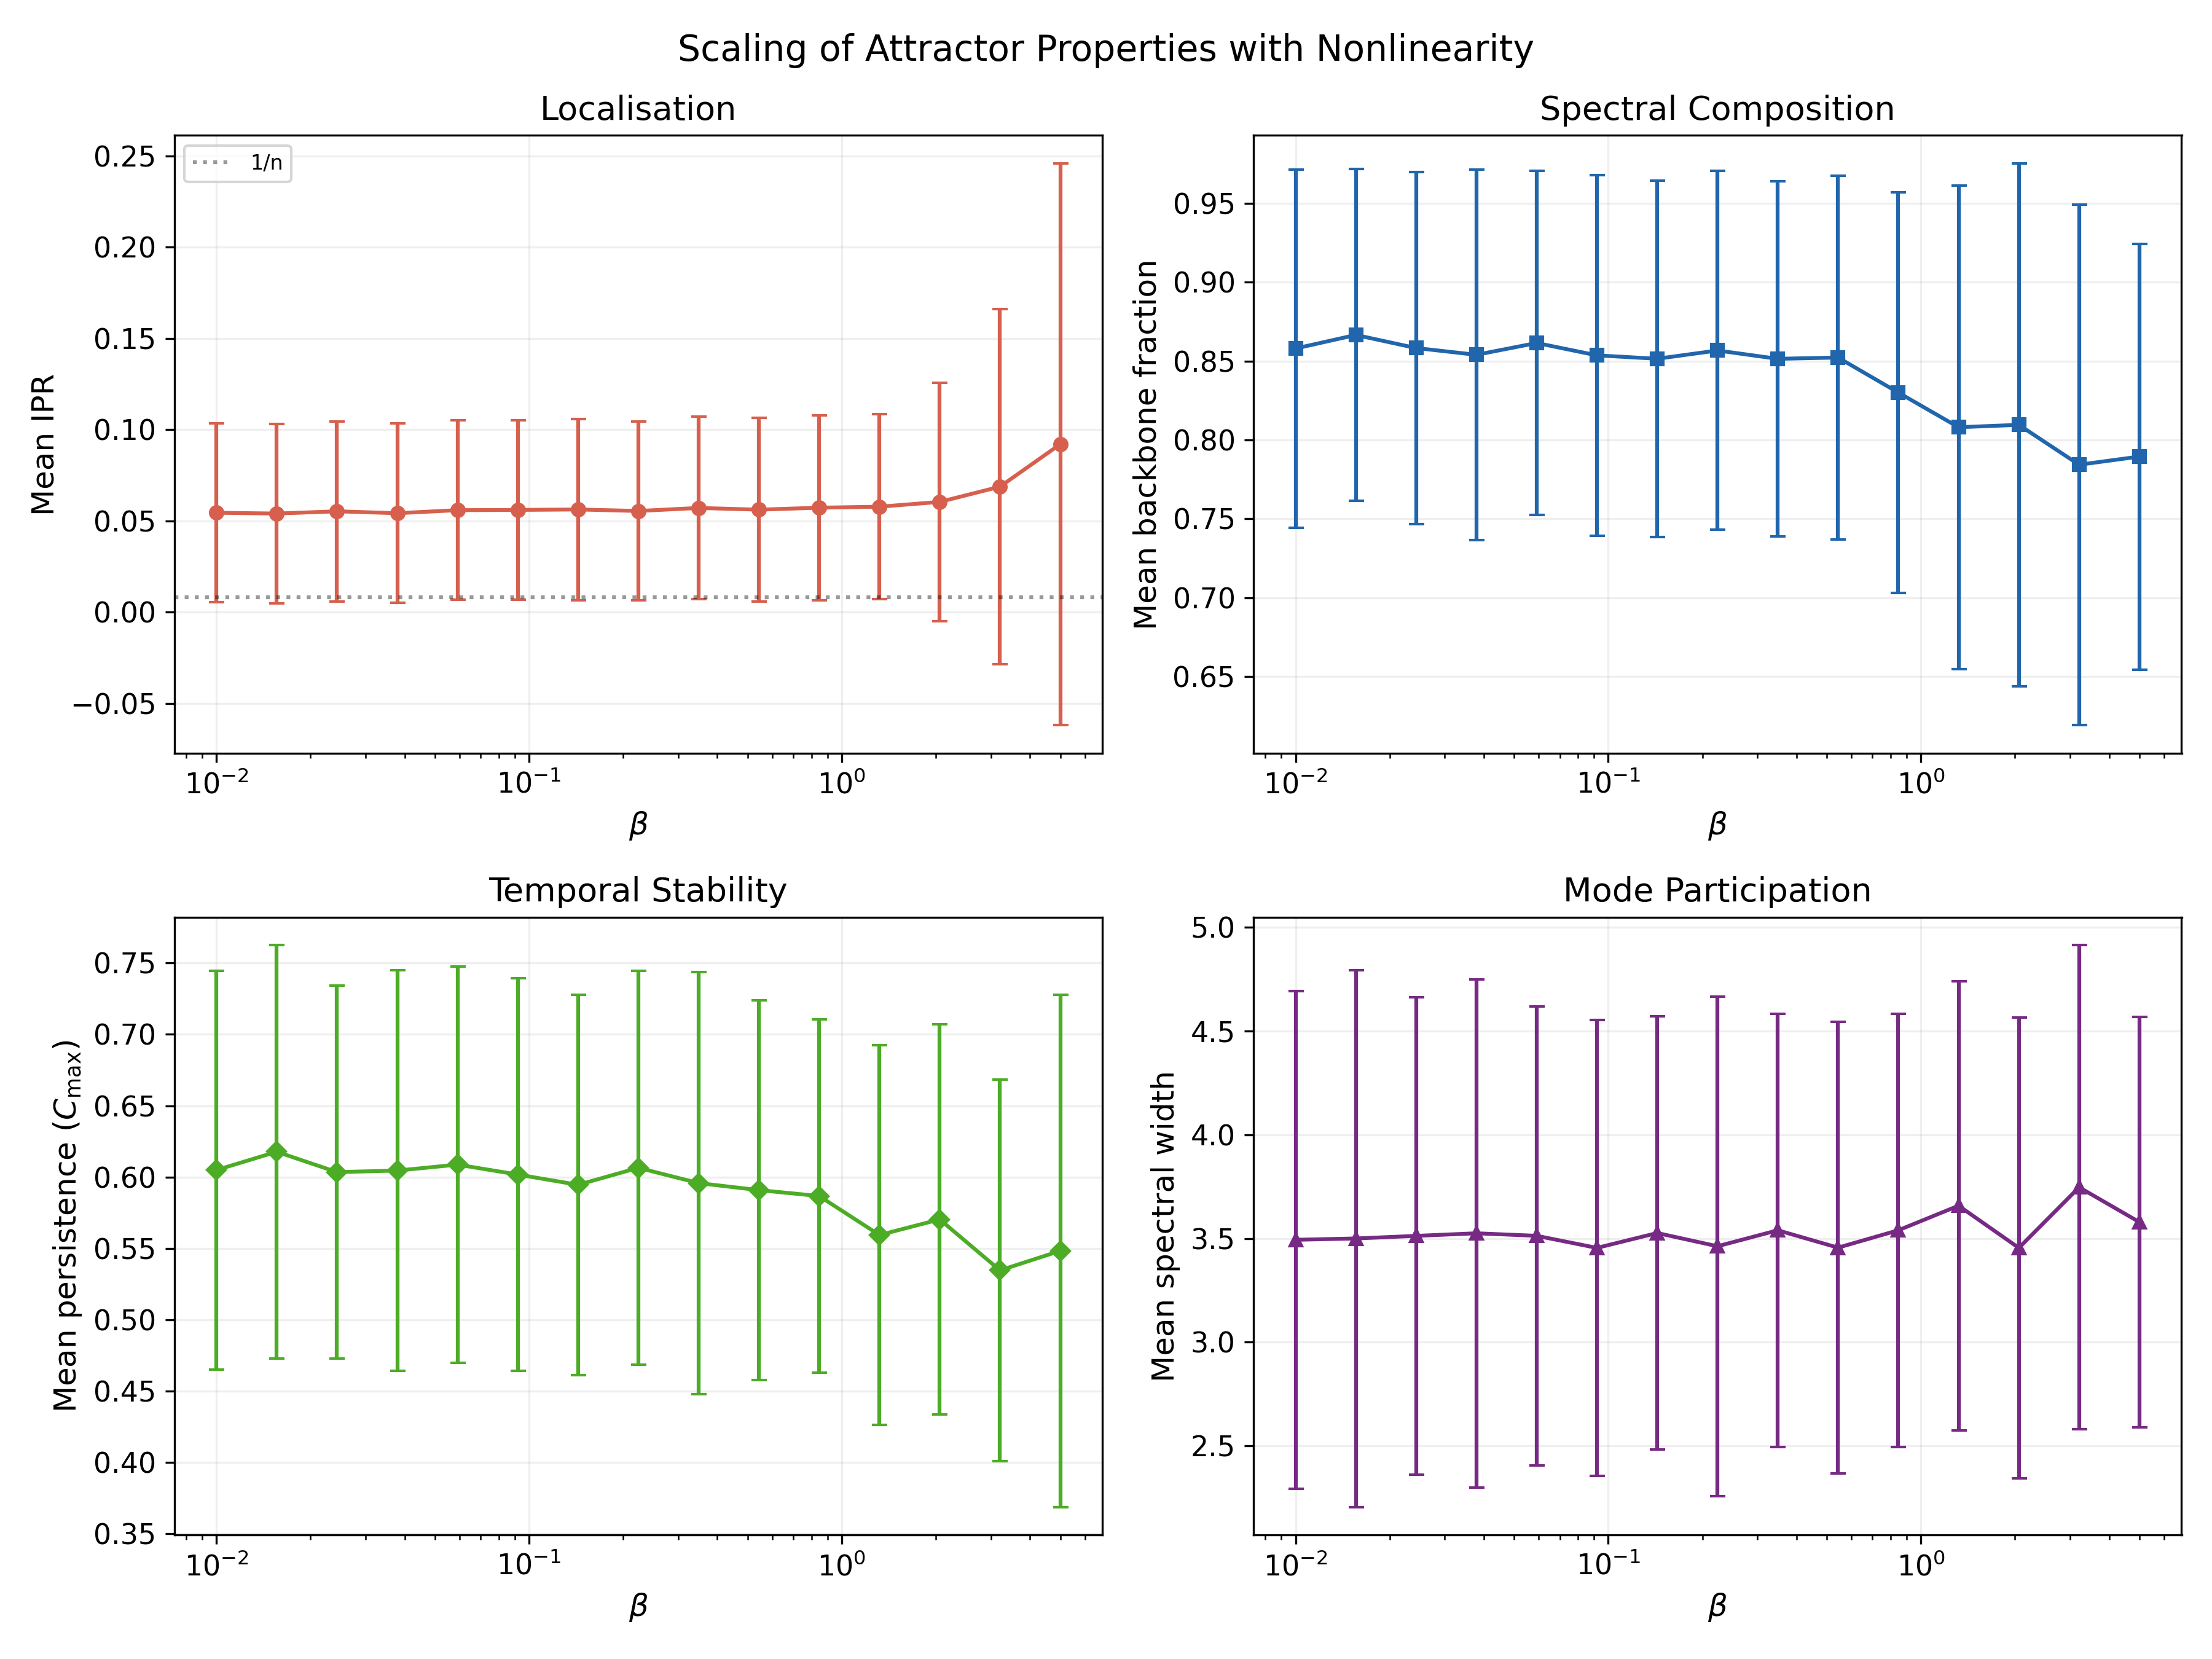
\includegraphics[width=0.95\textwidth]{fig_scaling_relations.png}
\caption{Scaling of attractor properties with nonlinear
strength~$\beta$.  Top left: mean IPR (localisation).  Top right:
mean backbone fraction.  Bottom left: mean persistence.  Bottom
right: mean spectral width.  Error bars show $\pm 1\sigma$ across
the ensemble at each~$\beta$.}
\label{fig:scaling}
\end{figure}

At low~$\beta$, attractors are dominated by backbone harmonic modes,
with low spectral width and low IPR.  As $\beta$ increases,
multi-mode interactions become more prevalent, leading to broader
spectral participation and increased localisation.  At higher~$\beta$,
localised breather-like states become more common, characterised by
high IPR and reduced persistence relative to backbone-dominated
states.

Importantly, these changes occur smoothly with~$\beta$, indicating
that the attractor structure evolves continuously rather than through
abrupt transitions.  This behaviour indicates that the organisation
of the attractor space is not static but follows reproducible scaling
relations with respect to the system's nonlinearity.


% ══════════════════════════════════════════════════════════
\section{Invariant Relationships}\label{sec:relationships}
% ══════════════════════════════════════════════════════════

Beyond individual distributions, we examine pairwise relationships
between the key quantities defining the attractor space
(Figures~\ref{fig:invariant} and~\ref{fig:corr}).

\begin{figure}[H]
\centering
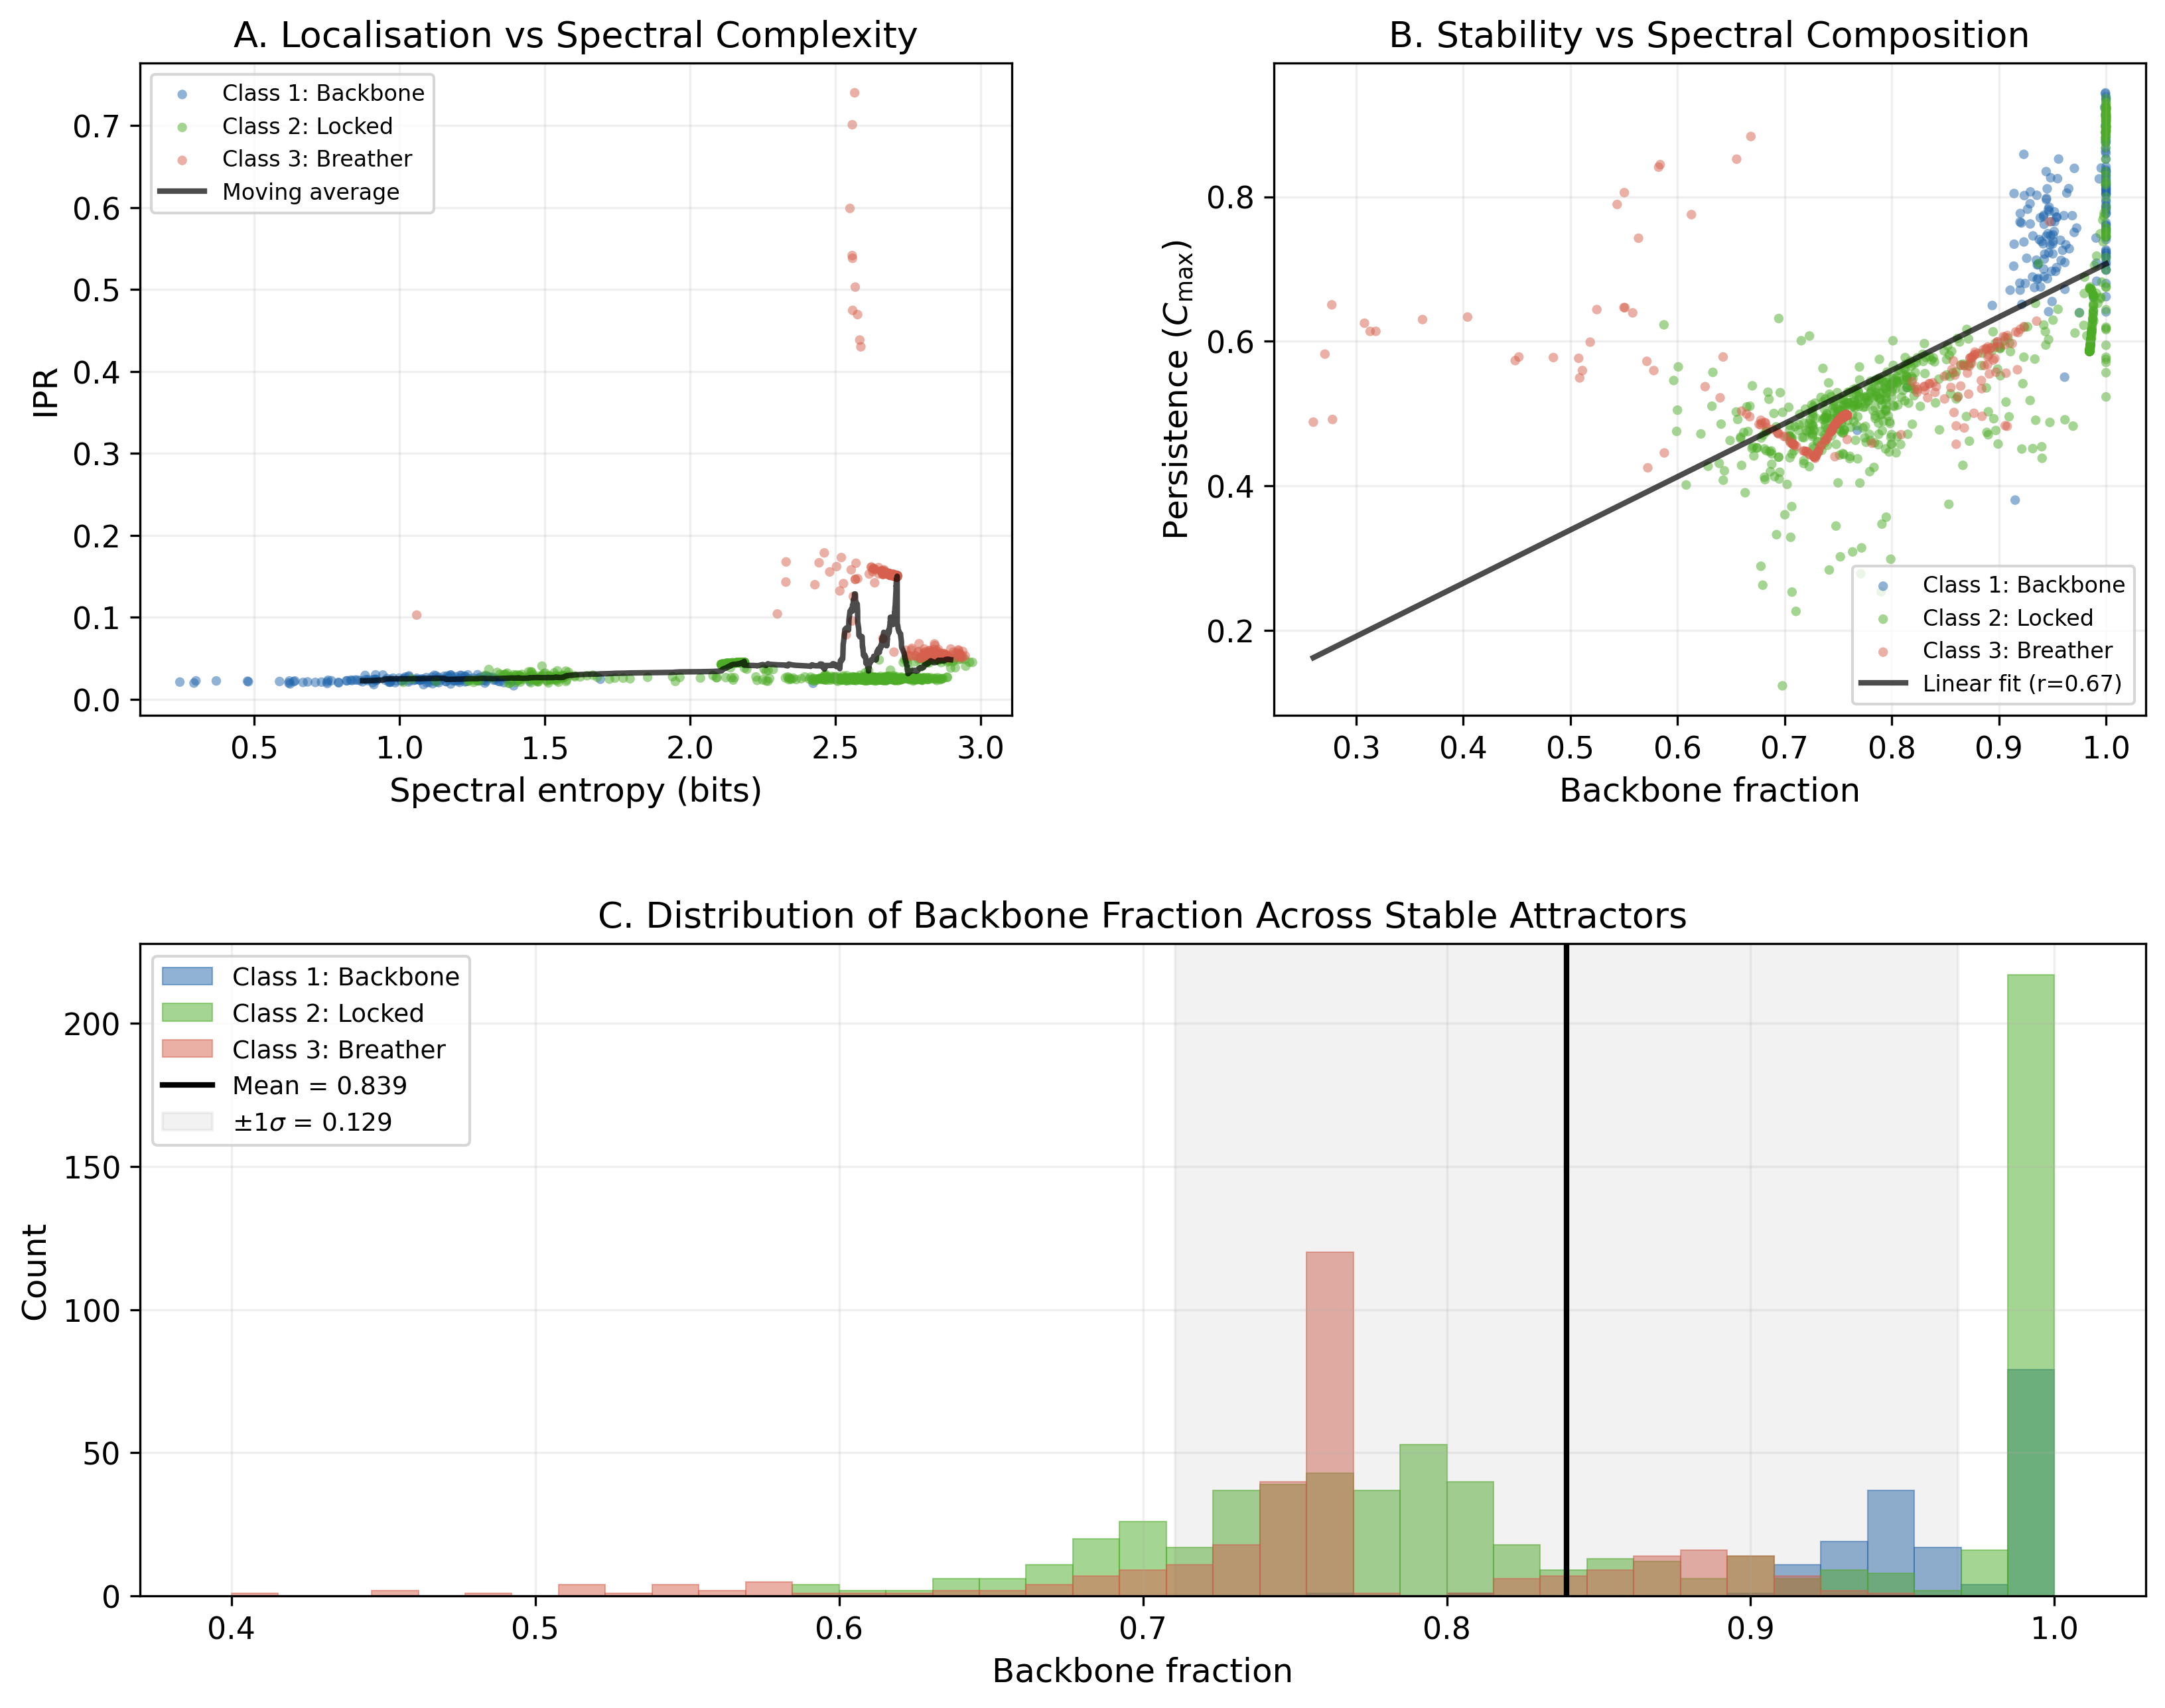
\includegraphics[width=0.95\textwidth]{fig_invariant_structure.png}
\caption{Invariant structure of the attractor space.
\emph{Panel~A:} IPR vs spectral entropy, coloured by attractor class.
The moving average (black) shows a systematic increase in
localisation with spectral complexity.
\emph{Panel~B:} Persistence vs backbone fraction.  The linear fit
(Spearman $r = 0.67$) shows that backbone-dominated attractors are
more temporally stable.
\emph{Panel~C:} Distribution of backbone fraction across all
1165~stable attractors.  The distribution concentrates at
$0.84 \pm 0.13$ (black line: mean; grey band: $\pm 1\sigma$).
These relationships are observed across the ensemble and are not
imposed by the classification procedure.}
\label{fig:invariant}
\end{figure}

\subsection{Localisation vs Spectral Complexity}

Localisation (IPR) increases systematically with spectral entropy
(Spearman $r = 0.47$, $p < 10^{-63}$;
Figure~\ref{fig:invariant}, Panel~A).  Attractors involving more
active sectors tend to exhibit higher IPR, indicating a coupling
between spectral complexity and spatial concentration.

This relationship is consistent with the mechanism described in
Part~III: broader spectral participation allows constructive
interference patterns that can produce localised configurations.

\subsection{Persistence vs Backbone Dominance}

Persistence correlates strongly with backbone fraction (Spearman
$r = 0.79$, $p < 10^{-250}$; Figure~\ref{fig:invariant}, Panel~B).
Attractors with a higher fraction of energy in backbone sectors
exhibit greater temporal stability.

The relationship is approximately monotonic: backbone fraction values
above $0.9$ correspond to persistence values above $0.7$, while
backbone fractions below $0.6$ are associated with persistence below
$0.4$.  This correlation is the strongest observed in the attractor
space and is consistent with the stability hierarchy reported in
Part~IV.

\subsection{Localisation--Persistence Trade-off}

IPR and persistence are negatively correlated (Spearman
$r = -0.27$, $p < 10^{-20}$), indicating a trade-off between spatial
concentration and temporal stability.  Highly localised attractors
(Class~3) tend to be less temporally persistent than extended
backbone-dominated states (Class~1), though both are classified as
stable within the observation window.

\begin{figure}[H]
\centering
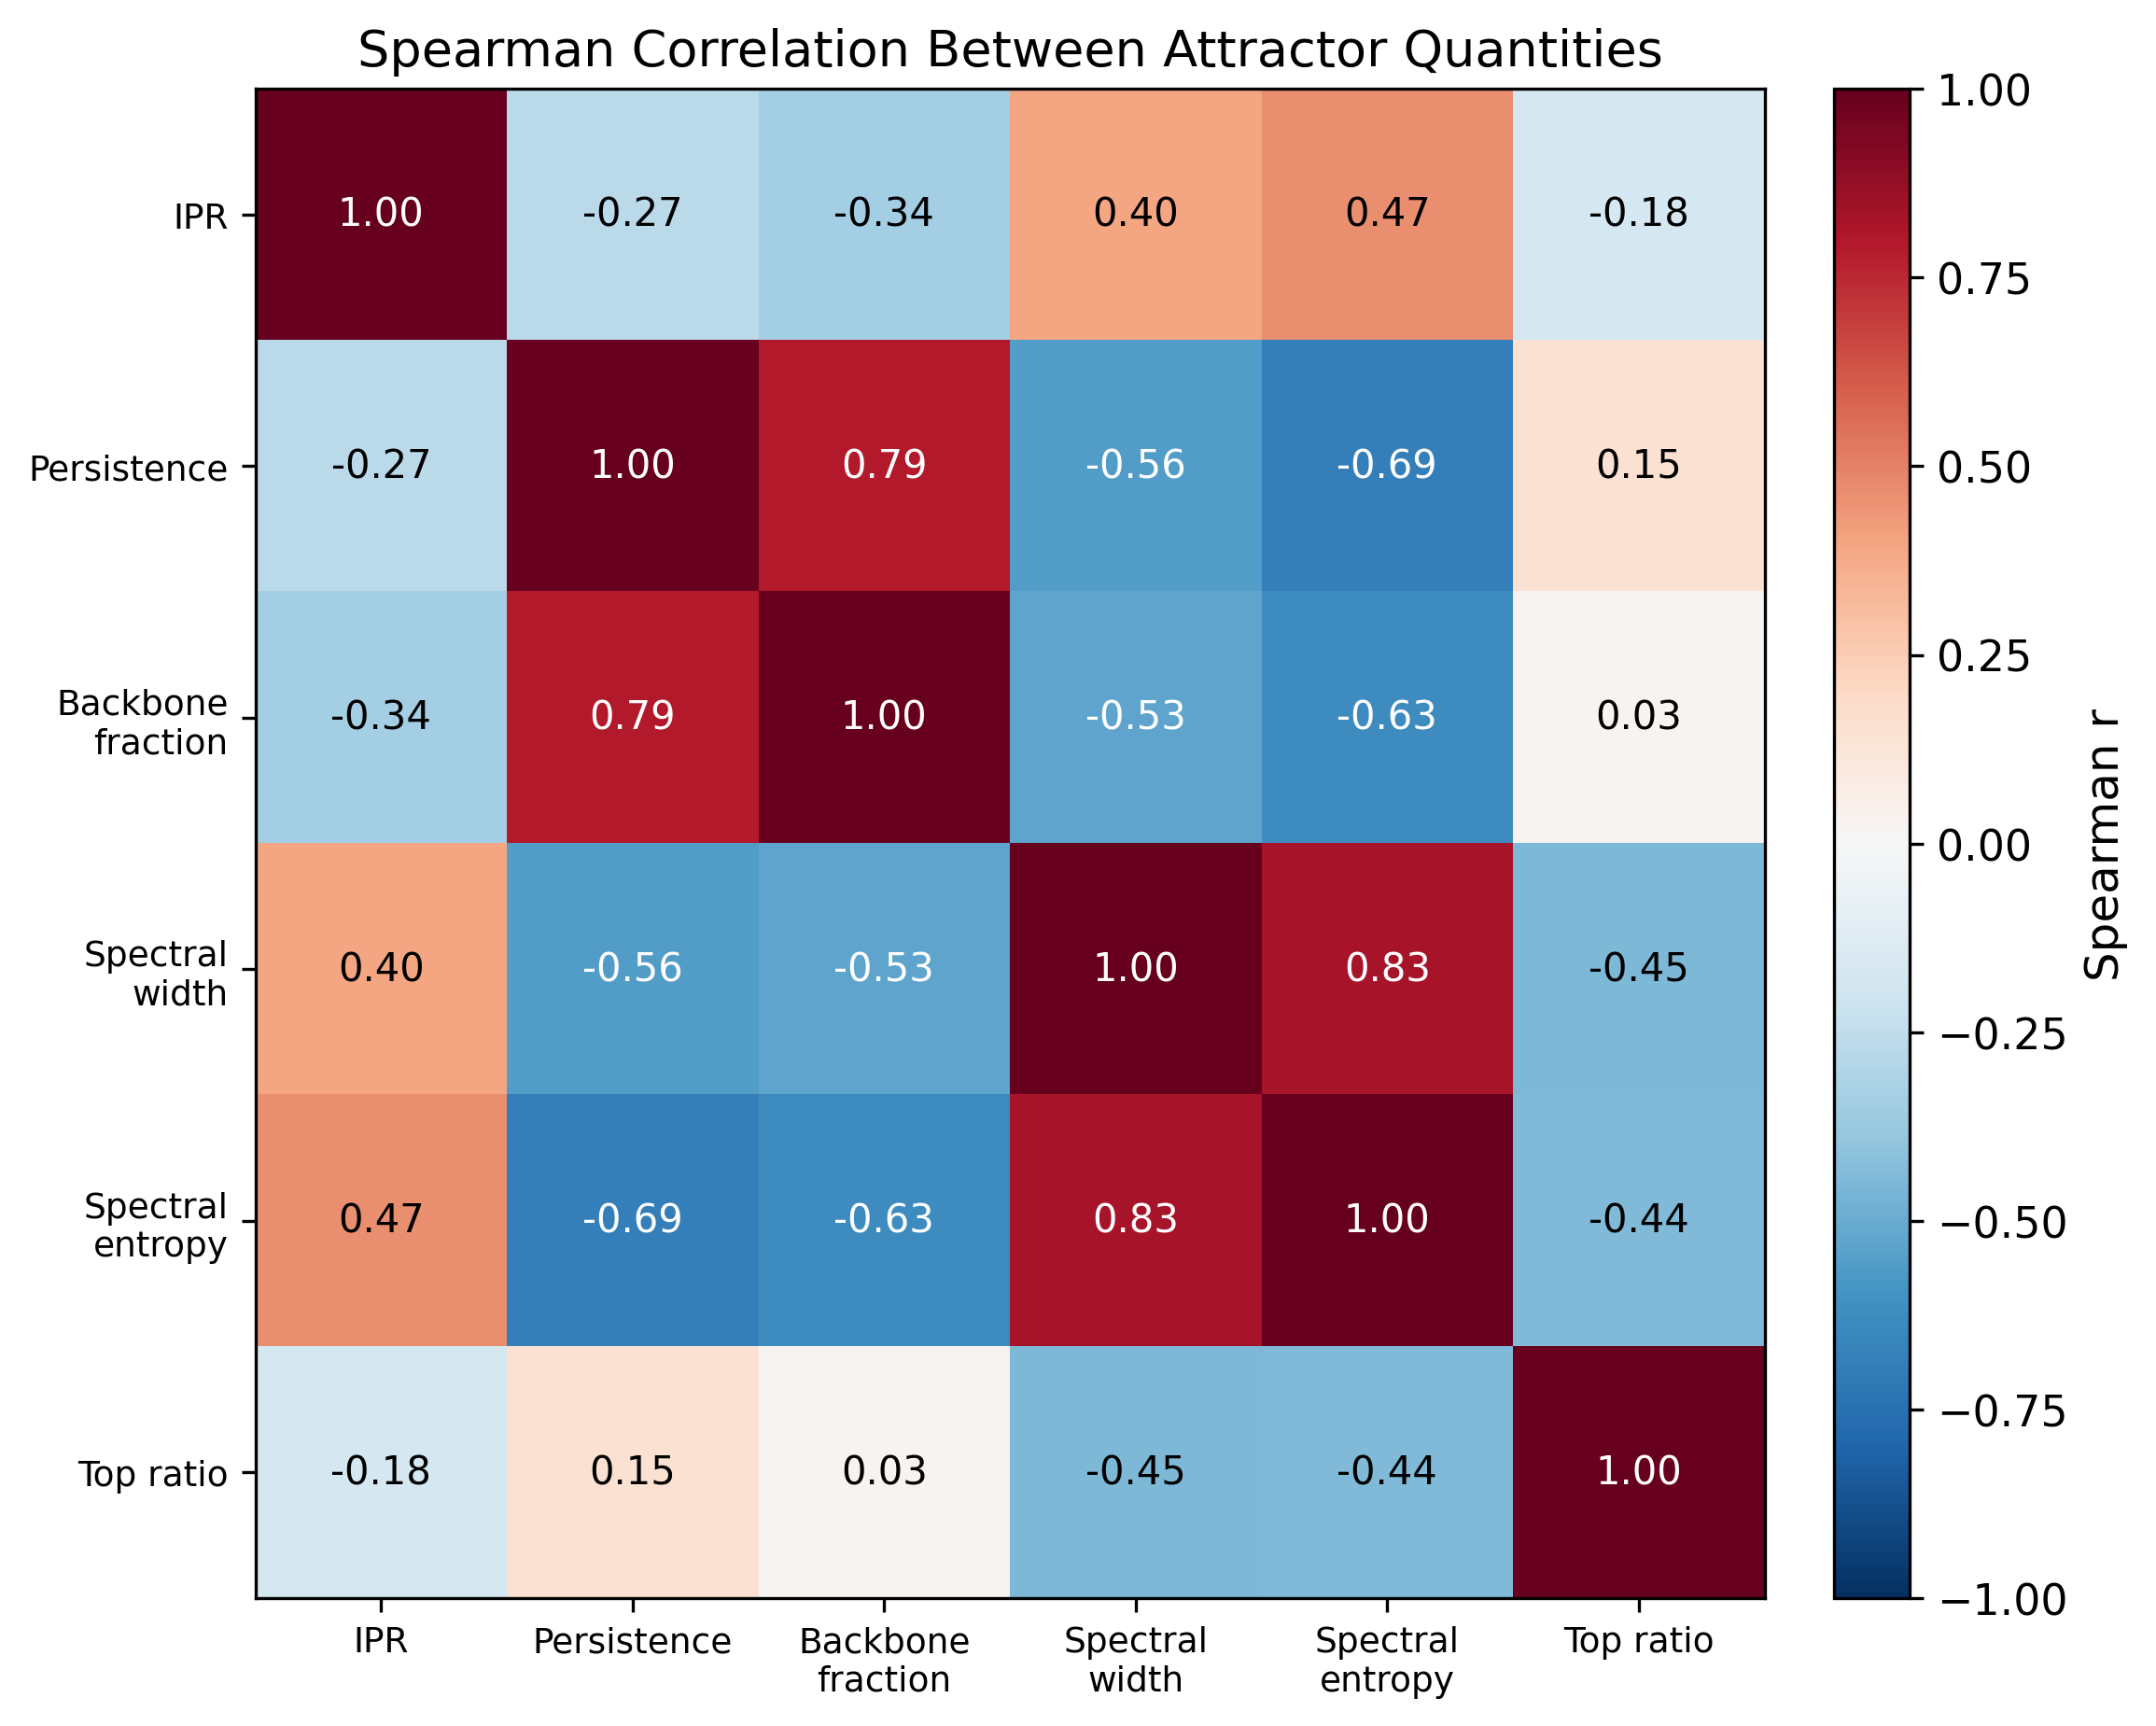
\includegraphics[width=0.85\textwidth]{fig_correlation_matrix.png}
\caption{Spearman rank correlation matrix between attractor
quantities.  Values indicate Spearman rank correlation between attractor
quantities across the full ensemble of 1165~stable attractors.
The strongest correlation is between persistence and backbone
fraction ($r = 0.79$).  IPR correlates positively with spectral
entropy ($r = 0.47$) and negatively with persistence ($r = -0.27$).}
\label{fig:corr}
\end{figure}

All reported correlations are statistically significant
($p < 10^{-20}$ in each case).

Taken together, these results indicate that the attractor space
exhibits internal relationships between spectral composition,
localisation, and stability.  These relationships are not imposed
by the classification procedure but emerge from the underlying
dynamics.


% ══════════════════════════════════════════════════════════
\section{Geometry--Spectrum Correspondence}\label{sec:geometry}
% ══════════════════════════════════════════════════════════

We examine whether the spatial and spectral properties of attractors
are independently distributed or exhibit structured correspondence
(Figure~\ref{fig:geom}).

\begin{figure}[H]
\centering
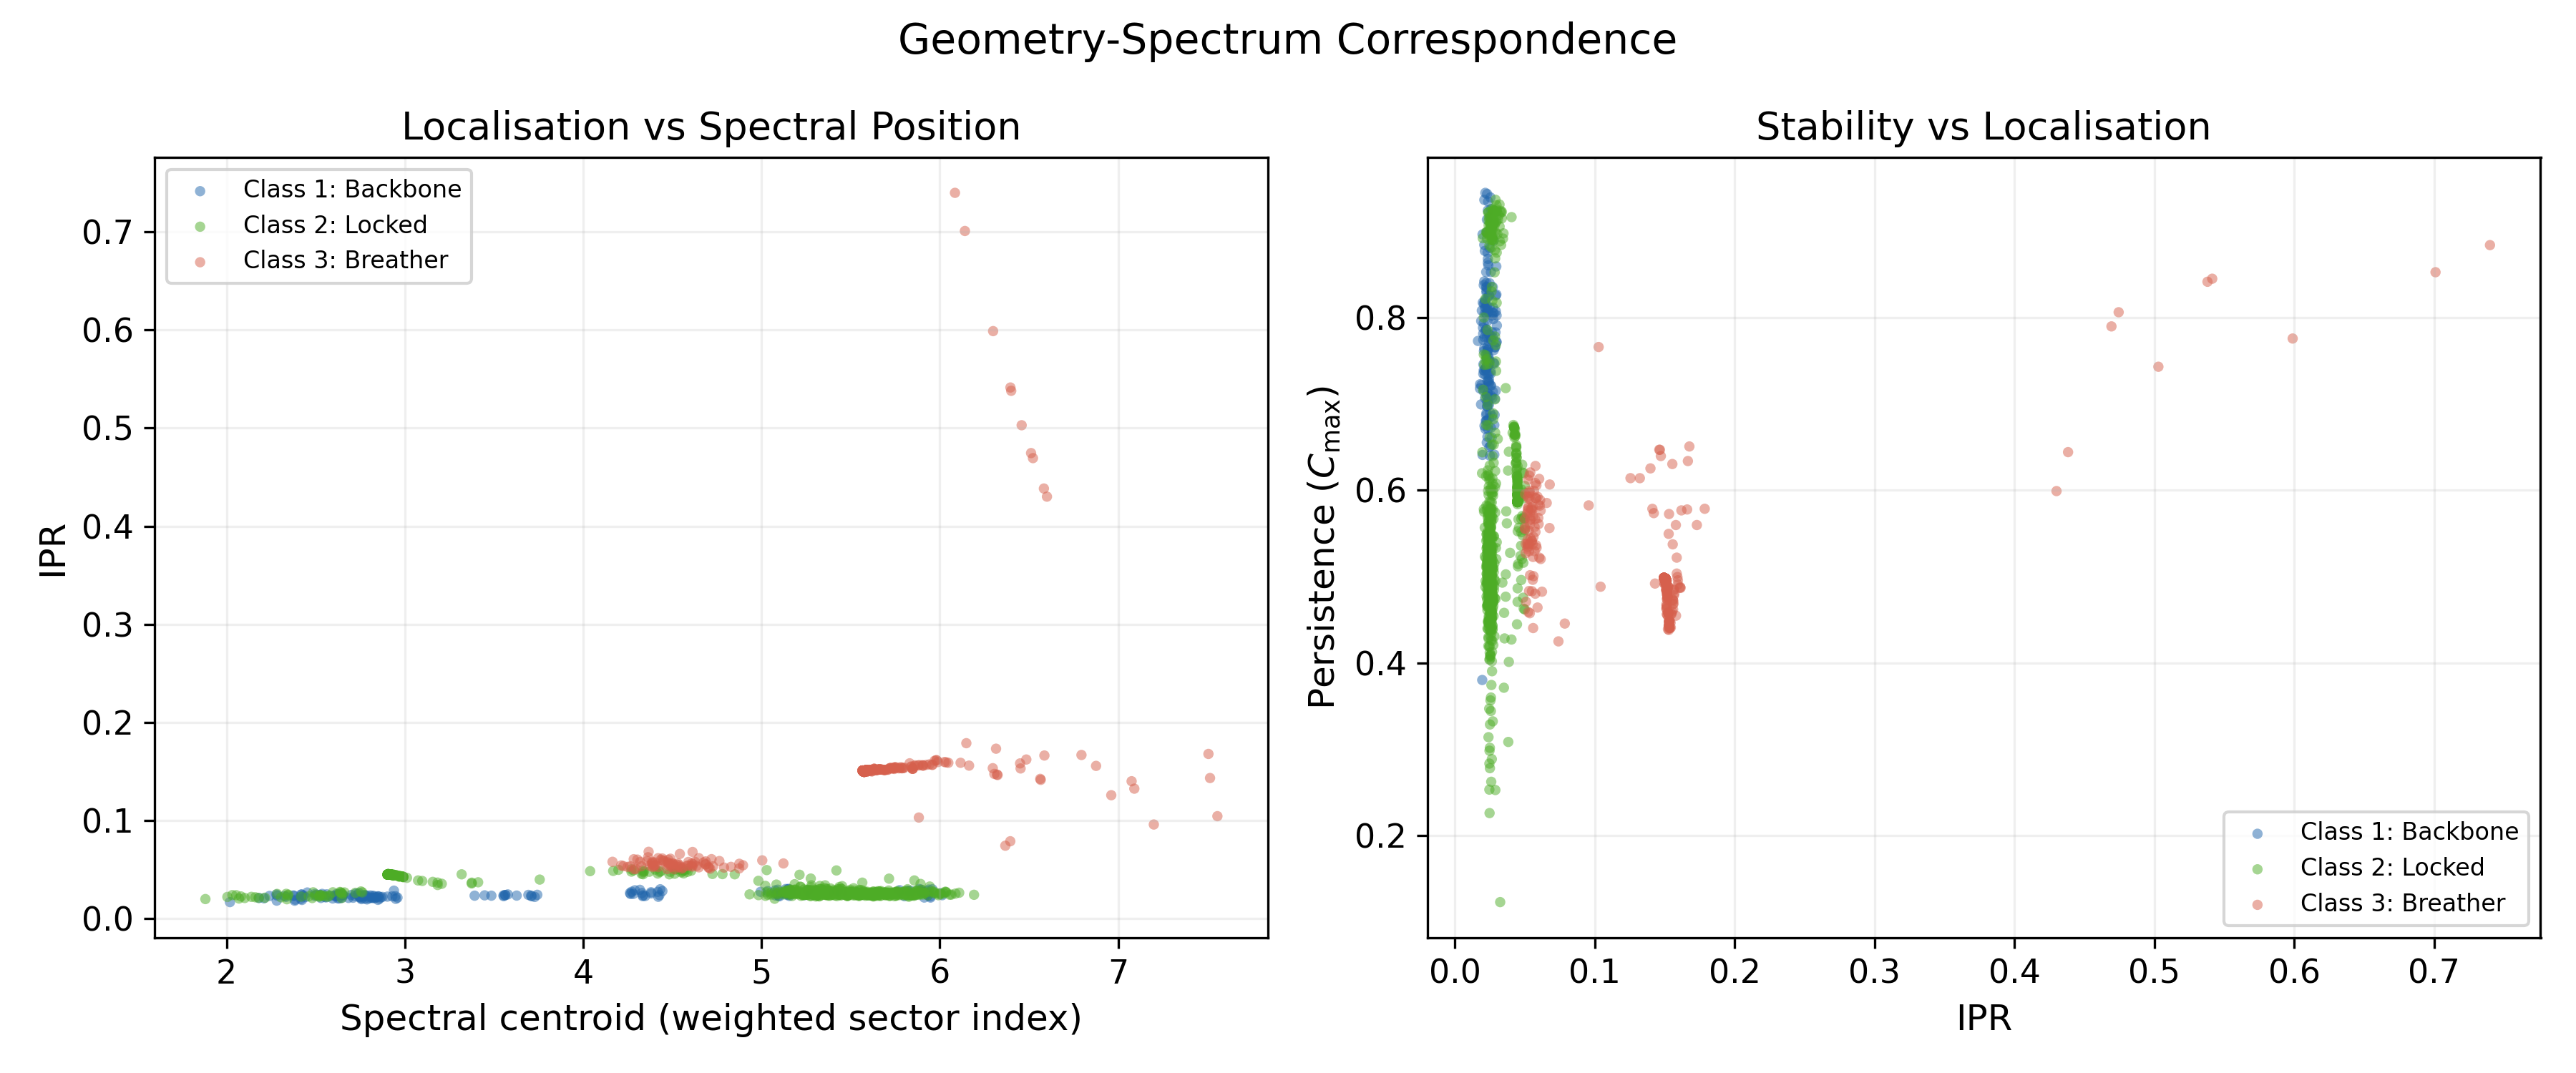
\includegraphics[width=0.95\textwidth]{fig_geometry_spectrum.png}
\caption{Geometry--spectrum correspondence.  Left: IPR vs spectral
centroid (weighted mean sector index), showing that localised
attractors tend to have higher spectral centroids.  Right:
persistence vs IPR, showing the localisation--persistence trade-off
across attractor classes.}
\label{fig:geom}
\end{figure}

Spatial and spectral properties are not independent but exhibit
structured correspondence.  Localised attractors (high IPR) tend
to involve higher-index spectral sectors (higher spectral centroid),
while extended attractors concentrate in the lower backbone sectors.
This is consistent with the observation from Part~IV that departure
sectors participate primarily in spatially localised configurations.


% ══════════════════════════════════════════════════════════
\section{Synthesis}\label{sec:synthesis}
% ══════════════════════════════════════════════════════════

The analyses of Sections~\ref{sec:invariants}--\ref{sec:geometry}
reveal that the attractor space of the $\Hfour$ system, within the
explored parameter range, is not merely constrained (as established
in Part~IV) but quantitatively organised.

The key findings are:

\begin{enumerate}[nosep]
\item The backbone fraction concentrates at $0.84 \pm 0.13$,
  indicating a preferred spectral composition rather than uniform
  coverage.

\item Persistence correlates strongly with backbone dominance
  ($r = 0.79$), establishing a quantitative link between spectral
  composition and temporal stability.

\item Localisation increases with spectral complexity ($r = 0.47$),
  indicating that spatial concentration and mode participation are
  coupled.

\item A localisation--persistence trade-off ($r = -0.27$) suggests
  competing organising mechanisms.

\item All relationships evolve smoothly with~$\beta$, following
  reproducible scaling relations.
\end{enumerate}

The existence of stable invariant relationships within the attractor
space suggests that the system may be governed by an organising
structure that extends beyond local nonlinear interactions.  While
these results remain purely dynamical, they indicate that the
$\Hfour$ system exhibits internal coherence at the level of its
attractor ensemble, within the explored parameter range.


% ══════════════════════════════════════════════════════════
\section{Discussion}\label{sec:discussion}
% ══════════════════════════════════════════════════════════

\subsection{Quantitative Organisation}

The results presented here indicate that the attractor space of the
$\Hfour$ system is not characterised by random dynamics, nor merely
by the existence of constraints (Part~IV), but by reproducible
quantitative relationships between spectral, spatial, and temporal
properties.

The strongest relationship---the persistence--backbone correlation
($r = 0.79$)---is consistent with the spectral backbone invariant
of Part~II: the 91-mode backbone provides a stable dynamical
subspace, and attractors confined to this subspace are more temporally
persistent.

\subsection{Relation to Previous Parts}

The invariant relationships identified here are consistent with the
structural progression of the series:

\begin{center}
\begin{tabular}{@{}ll@{}}
Part~I   & establishes the phenomenon \\
Part~II  & establishes the spectral structure \\
Part~III & establishes the attractor taxonomy \\
Part~IV  & establishes the selection rules \\
Part~V   & establishes the invariant relationships \\
\end{tabular}
\end{center}

Each successive paper identifies a deeper layer of organisation
within the same dynamical system.  The invariant relationships of the
present work are consistent with, and appear to follow from, the
spectral invariants and selection rules of the preceding papers.

\subsection{Scope}

These results are presented as properties of a nonlinear dynamical
system on a structured graph and do not assume any direct mapping to
physical observables.  The invariant relationships are empirical and
derived from numerical simulation.  The term ``invariant'' is used
here to denote quantities with low variance across the attractor
ensemble, not in the formal mathematical sense of a conserved
quantity.


% ══════════════════════════════════════════════════════════
\section{Limitations}\label{sec:limitations}
% ══════════════════════════════════════════════════════════

The present results are numerical and do not constitute analytical
derivations of the observed relationships.

Limitations include:
\begin{itemize}[nosep]
\item \textbf{Finite sampling:} the ensemble of 1165~stable
  attractors provides coverage but may not capture all attractor
  families.
\item \textbf{Parameter dependence:} all results are obtained at
  fixed $\omega_0 = 1$ and $\lambda = 1$.
\item \textbf{Correlation vs causation:} the observed correlations
  do not establish causal relationships.  The strong
  persistence--backbone correlation may reflect a common underlying
  cause (spectral confinement) rather than a direct mechanism.
\item \textbf{Threshold dependence:} the spectral width depends on
  the activation threshold $\theta = 0.10$.
\item \textbf{No analytical derivation:} the invariant relationships
  are empirical observations; derivation from the $\Hfour$ algebra
  remains an open problem.
\end{itemize}


% ══════════════════════════════════════════════════════════
\section{Outlook}\label{sec:outlook}
% ══════════════════════════════════════════════════════════

Future work should focus on:
\begin{itemize}[nosep]
\item analytical derivation of the persistence--backbone relationship
  from the spectral properties of the Laplacian;
\item investigation of whether the observed invariants hold under
  modified dynamics (different nonlinearities, dissipation);
\item extension to coupled $\Hfour$ systems and the $\Eeight$ root
  polytope;
\item formal characterisation of the attractor space as a
  low-dimensional manifold within the full phase space.
\end{itemize}


% ══════════════════════════════════════════════════════════
\section{Conclusion}\label{sec:conclusion}
% ══════════════════════════════════════════════════════════

The attractor space of the nonlinear field system on the 600-cell
vertex graph exhibits reproducible quantitative relationships between
spectral composition, spatial localisation, and temporal persistence.
The backbone fraction concentrates at $0.84 \pm 0.13$ across
1165~stable attractors.  Persistence correlates with backbone
dominance (Spearman $r = 0.79$), localisation increases with spectral
complexity ($r = 0.47$), and these relationships evolve smoothly
with~$\beta$.

Together with the preceding papers, these results indicate that the
$\Hfour$ spectral algebra appears to organise nonlinear dynamics at
multiple levels: from spectral structure (Part~II) through attractor
classification (Part~III) and selection rules (Part~IV) to
reproducible invariant relationships within the attractor space
(Part~V).  No physical interpretation is required for or assumed in
these conclusions.

\paragraph{Reproducibility.}
All analyses use the attractor ensemble from Part~IV.  Code and
parameters are specified in the accompanying repository.


% ══════════════════════════════════════════════════════════
% References
% ══════════════════════════════════════════════════════════
\begin{thebibliography}{10}

\bibitem{paper1}
L.~Smart,
``Symmetry-Constrained Resonant Modes on $H_4$ Geometry,''
\textit{VFD Working Paper Series}, WO-VFD-PAPER-001, 2025.

\bibitem{paper2}
L.~Smart,
``Algebraic Invariants of the $H_4$ Laplacian Spectrum,''
\textit{VFD Working Paper Series}, WO-VFD-PAPER-002, 2025.

\bibitem{paper3}
L.~Smart,
``Nonlinear Mode Localisation on the $H_4$ Graph,''
\textit{VFD Working Paper Series}, WO-VFD-PAPER-003, 2026.

\bibitem{paper4}
L.~Smart,
``Selection Rules and Constraints on Nonlinear Attractors
in the $H_4$ System,''
\textit{VFD Working Paper Series}, WO-VFD-PAPER-004, 2026.

\bibitem{flach2008}
S.~Flach and A.~V.~Gorbach,
``Discrete breathers --- Advances in theory and applications,''
\textit{Physics Reports} \textbf{467}, 1--116, 2008.

\bibitem{humphreys1990}
J.~E.~Humphreys,
\textit{Reflection Groups and Coxeter Groups}.
Cambridge University Press, 1990.

\bibitem{coxeter1973}
H.~S.~M.~Coxeter,
\textit{Regular Polytopes}, 3rd~ed.
Dover Publications, 1973.

\bibitem{chung1997}
F.~R.~K.~Chung,
\textit{Spectral Graph Theory}.
AMS, 1997.

\end{thebibliography}

\vfill
\noindent\rule{\textwidth}{0.4pt}\\[4pt]
{\footnotesize
\textit{Vibrational Field Dynamics Working Paper Series}
\hfill Part~V \quad v1.1 (final-hardened)}

\end{document}
